\documentclass{robinminion}

\usepackage[round]{natbib}
\bibliographystyle{plainnat}

\usepackage{rotating, amsthm}

\author{Willem Heijltjes and Robin Houston}
\title{The proof equivalence problem for multiplicative linear logic is \textsc{pspace}-complete v0.2}

\def\mkspin#1#2{\smash{%
  \rotatebox[origin=c]{180}{\mathsurround=0pt$#1#2$}}}
\def\spin{\mathpalette\mkspin}
\def\parr{\mathbin{\spin{\&}}}
\let\tn\otimes

\newtheorem{lemma}{Lemma}

\begin{document}

\maketitle

\linespread{1.1}\selectfont
\noindent\emph{\textsc{mll} proof equivalence} is the problem of deciding whether one proof may be turned into another by a series of commuting conversions. Thanks to many years of work on proof nets \citep{Girard87, DR89, TrimbleThesis, BCST, HughesFreeStar} we know this is equivalent to a reasonably simple rewiring problem on graphs.

On the other side of the fence, thanks to many years of work on combinatorial games and complexity theory \citep{RushHour, HearnDemaineTCS, GamesPuzzlesAndComputation, TheConnectivityOfBooleanSatisfiability, ReconfigurationProblems} we know many examples of rewiring problems on graphs that are \textsc{pspace}-complete. So in a sense it is not a great surprise to find that \textsc{mll} proof equivalence is \textsc{pspace}-complete as well. On the other hand, I think this is the first time these different ideas have been brought together. We will give a reduction from the configuration-to-configuration problem for Nondeterministic Constraint Logic \citep{HearnDemaineTCS, GamesPuzzlesAndComputation}.


\section*{Nondeterministic Constraint Logic}

A \emph{constraint graph} is an undirected graph with an assignment of a natural number \emph{weight} to each edge and a natural number \emph{minimum in-flow constraint} to each vertex. A \emph{configuration} of the constraint graph is an orientation (direction) of the edges such that the sum of incoming edge weights at each vertex is at least the minimum in-flow constraint of that vertex. A \emph{move} from one configuration to another configuration consists of reversing the direction of a single edge such that the minimum in-flow constraints remain satisfied. The \emph{configuration-to-configuration problem} is: given a constraint graph and two configurations $s$ and $t$, is there a sequence of moves from $s$ that results in $t$ (or vice versa, since moves are reversible). This problem is \textsc{pspace}-complete. \citep{HearnDemaineTCS, GamesPuzzlesAndComputation}

For present purposes, we need to introduce a slightly different notion of configuration. A \emph{progressive configuration} assigns to each edge not only a direction but also an \emph{orientation value}, which is a natural number at most the weight of the edge. The configuration is valid when the sum of the incoming orientation values at each vertex is precisely the minimum in-flow constraint of that vertex. A move consists of:
\begin{itemize}
    \item either reversing the direction of an edge that has zero orientation value
    \item or taking a pair of edges oriented towards the same node, and incrementing the orientation value of one while decrementing the orientation value of the other.
\end{itemize}

Each progressive configuration determines a configuration in the Hearn-Demaine sense, and an edge of a progressive configuration may be reversed just when the edge of the corresponding Hearn-Demaine configuration may be. In this sense the notions are equivalent. We'll sometimes write \textsc{pncl} to mean \textsc{ncl} with progressive configurations.

\section*{Hughes-style proof nets}

We shall work in the unit-only fragment of \textsc{mll}, where our formulas are built from the constants $\bot$ and $1$ with the operations $\tn$ and $\parr$, and we'll work with one-sided sequents and modulo associativity of $\tn$ and $\parr$.

In this setting, a Hughes-style proof net for a given sequent is simply a function from the occurences of $\bot$ to the occurences of $1$ such that the usual proof net criterion is satisfied. A rewiring step consists of moving a single $\bot$-link to a different occurence of $1$.


\section*{Notation}

We'll use a diagrammatic notation for sequents and proof nets. The atoms $1$ and $\bot$ are represented by a circle $\circ$ and a disc $\bullet$ respectively. Then we build up larger expressions in the following way.
%
Suppose $A$ is represented by \raisebox{-0.3\height}{
\includegraphics[scale=0.75]{hex-A.pdf}}
and $B$ is represented by \raisebox{-0.3\height}{
\includegraphics[scale=0.75]{hex-B.pdf}};
%
then $A\parr B$ is \raisebox{-0.3\height}{
\includegraphics[scale=0.75]{hex-AparB.pdf}}
and $A\tn B$ is \raisebox{-0.3\height}{
\includegraphics[scale=0.75]{hex-AtnB.pdf}}.
%
Tensor of multiple elements is denoted by stringing them together in a line, so $A\tn B\tn C$ is
\raisebox{-0.3\height}{
\includegraphics[scale=0.75]{hex-AtnBtnC.pdf}}.
%
Boxes play the role of parentheses, so $(A\parr B)\tn C$ is drawn as \begin{center}{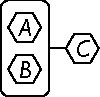
\includegraphics[scale=1]{hex-AparBtnC.pdf}}\end{center}

\noindent So, for example, this sequent
\[ \vdash \bot\tn\bot, \bot\tn\bot, \bot\tn\bot, \bot\tn\bot, 1, \{[(1\parr 1\parr 1)\tn(1\parr 1\parr 1)]\parr 1\parr (\bot\tn\bot\tn\bot)\parr 1\}\tn\bot \]
could be drawn like this:
\begin{center}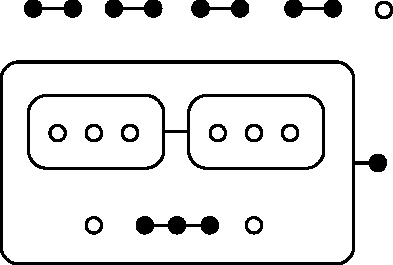
\includegraphics[scale=0.75]{example-sequent.pdf}\end{center}

\noindent We represent a proof net by drawing an arrow from each $\bullet$ to some $\circ$. For example, one proof net on the above sequent is
\begin{center}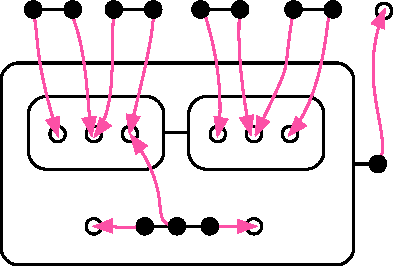
\includegraphics[scale=0.75]{example-sequent-proofnet.pdf}\end{center}

\noindent It will be useful to have an abbreviated notation for expressions of the form $\bot\tn\cdots\tn\bot$ and $1\parr\cdots\parr 1$. We shall write a larger disc with the number $i$ inside for the tensor of $i+1$ occurences of $\bot$, and a larger circle with $j$ inside for the par of $j+1$ occurences of $1$, like so:
\begin{center}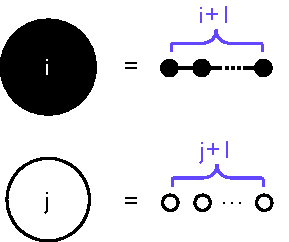
\includegraphics[scale=0.75]{abbreviated-notation.pdf}\end{center}

\noindent We also use fat arrows to represent a series of arrows in a proof net, like so:
\begin{center}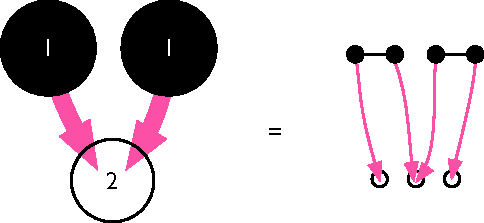
\includegraphics[scale=0.75]{fat-arrow-example.pdf}\end{center}

\noindent This is the reason for the `$+1$' in the definition: it means that a valid proof net is formed by a collection of fat arrows with a common target just when the numbers written on the sources add up to the number written on the target. The price we pay for this convenience is a less obvious arithmetic of decomposition:
\begin{center}
    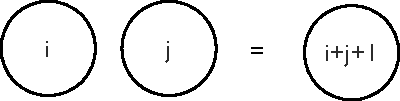
\includegraphics[scale=0.75]{decomposed-circles.pdf}\\[1em]
    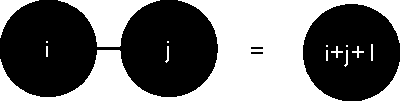
\includegraphics[scale=0.75]{decomposed-discs.pdf}
\end{center}

\section*{Reduction}

The idea is to encode a constraint graph as a sequent, in such a way that proof nets over the sequent correspond to progressive configurations of the constraint graph, and each \textsc{pncl} move corresponds to a sequence of rewiring steps in the proof net. First we number the nodes from $0$ to $n$, and let $k$ be the number of edges. Then we represent node $i$ with minimum inflow constraint $c$ by the following gadget:
\begin{center}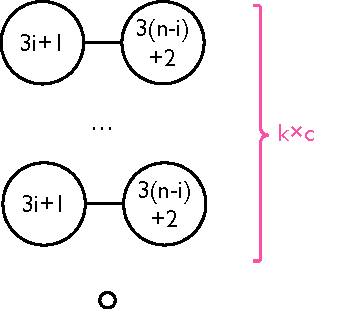
\includegraphics[scale=0.75]{node-gadget.pdf}\end{center}

\noindent and an edge of weight $w$ connecting nodes $i < j$ by the following:
\begin{center}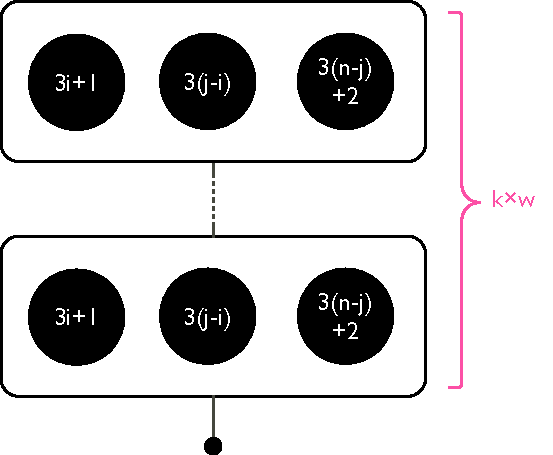
\includegraphics[scale=0.75]{edge-gadget.pdf}\end{center}

\noindent The other gadget we need is the ``edge absorber'':
\begin{center}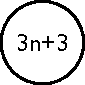
\includegraphics[scale=0.75]{edge-absorber-gadget.pdf}\end{center}

\noindent
The key property of this encoding is that a row of an edge gadget may be attached completely to a row of a node gadget just when the edge is attached to that node in the constraint graph, as follows:
\begin{center}
    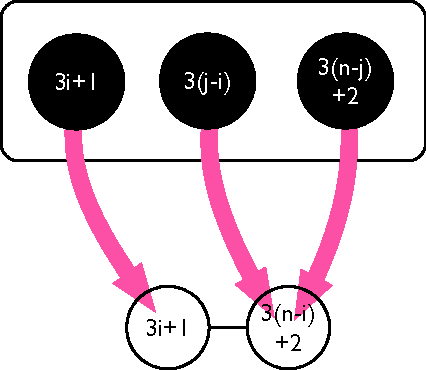
\includegraphics[scale=0.75]{attached-gadgets-i.pdf}\hskip2em
    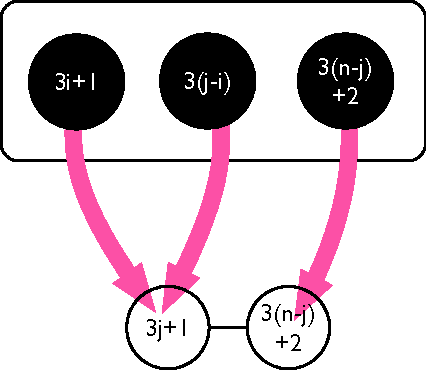
\includegraphics[scale=0.75]{attached-gadgets-j.pdf}
\end{center}
\noindent Similarly, a row of any edge gadget may be attached completely to an edge absorber:
\begin{center}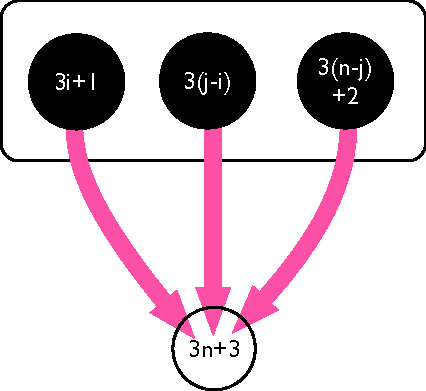
\includegraphics[scale=0.75]{attached-edge-absorber.pdf}\end{center}

\noindent Let $d$ be the difference between the sum of the edge weights and the sum of the minimum inflow constraints.
Our sequent consists of:
\begin{itemize}
    \item All the edge gadgets (as separate entries),
    \item The tensor of all the node gadgets (a single entry),
    \item $k\times d$ edge absorbers (as separate entries).
\end{itemize}

\noindent Now, every progressive configuration of the constraint graph may be represented by a proof net over this sequent, in the following way:
\begin{itemize}
    \item Each edge is attached to the the node it is oriented towards, by attaching the small $\bullet$ at the bottom of the edge gadget to the small $\circ$ at the bottom of the node gadget. We'll call this the \emph{index link}.
    \item $kv$ rows of the edge gadget are attached to $kv$ rows of the node gadget as described above, where $v$ is the edge's orientation value.
    \item The remaining edge weight is assigned to edge absorbers, one row of the edge gadget to a single edge absorber. In total an edge of weight $w$ and orientation value $v$ uses $k(w-v)$ edge absorbers.
\end{itemize}

\noindent Of course there are many proof nets over our sequent that are not precisely of this form. We shall try to establish xxxx things:
\begin{itemize}
	\item Every proof net over this sequent corresponds (in a sense we shall define precisely) to a slightly generalised form of progressive configuration;
	\item xxxx
	\item Every move in the \textsc{pncl} game may be simulated by some sequence of proof net rewirings.
	\item If we start with a proof net that represents a configuration $x$, then perform a sequence of rewirings and end up with another proof net that represents a different configuration $y$, then there is a sequence of \textsc{pncl} moves from $x$ to $y$.
\end{itemize}

However the converse is false: in general it is possible to simulate certain invalid moves as well. The next section describes how this can happen, and how to fix it.


\subsection*{Naughty proof nets}

\noindent Although it is clear that a row of the node gadget may be filled by an edge gadget only when the edge is attached to that node, it is possible for several edge gadgets to join forces and fill part of a node gadget illegitimately. For example, suppose we have the following constraint graph with four nodes
\begin{center}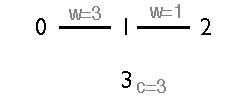
\includegraphics[scale=0.75]{naughty-constraint-graph.pdf}\end{center}
Then it is possible for the two edges to fill the gadget representing node 3 and one edge absorber. The relevant gadgets are these:
\begin{center}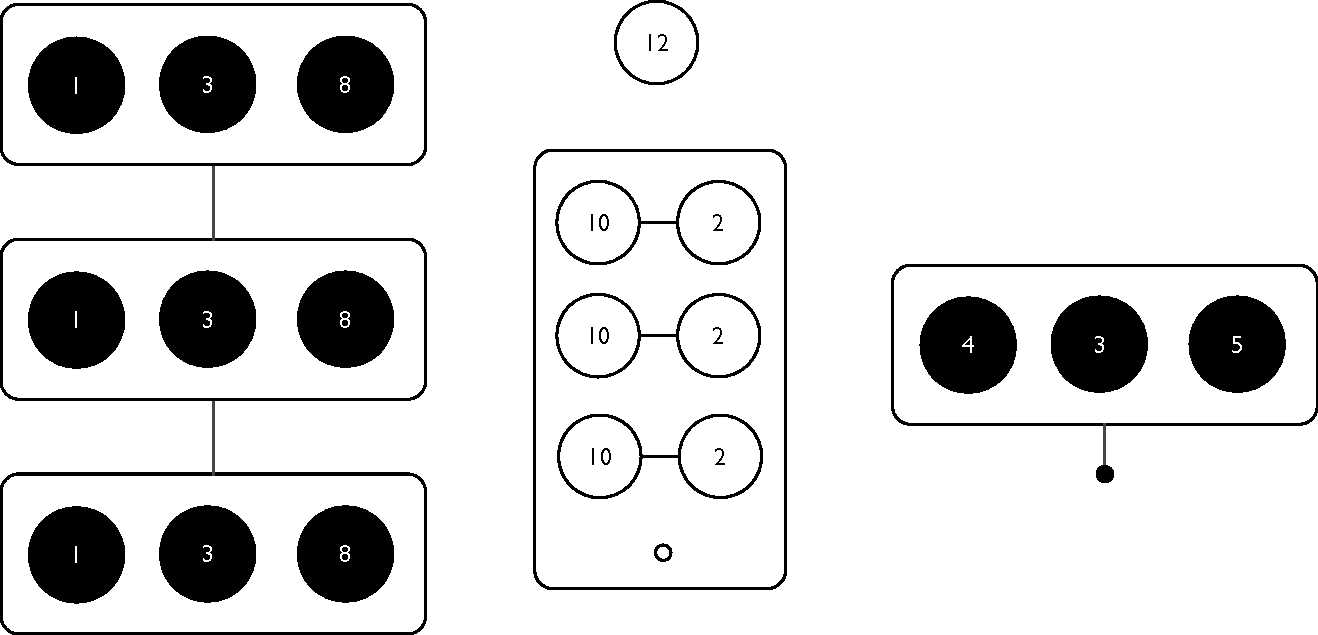
\includegraphics[scale=0.5]{naughty-gadgets.pdf}\end{center}
and one illegitimate wiring looks like this:
\begin{center}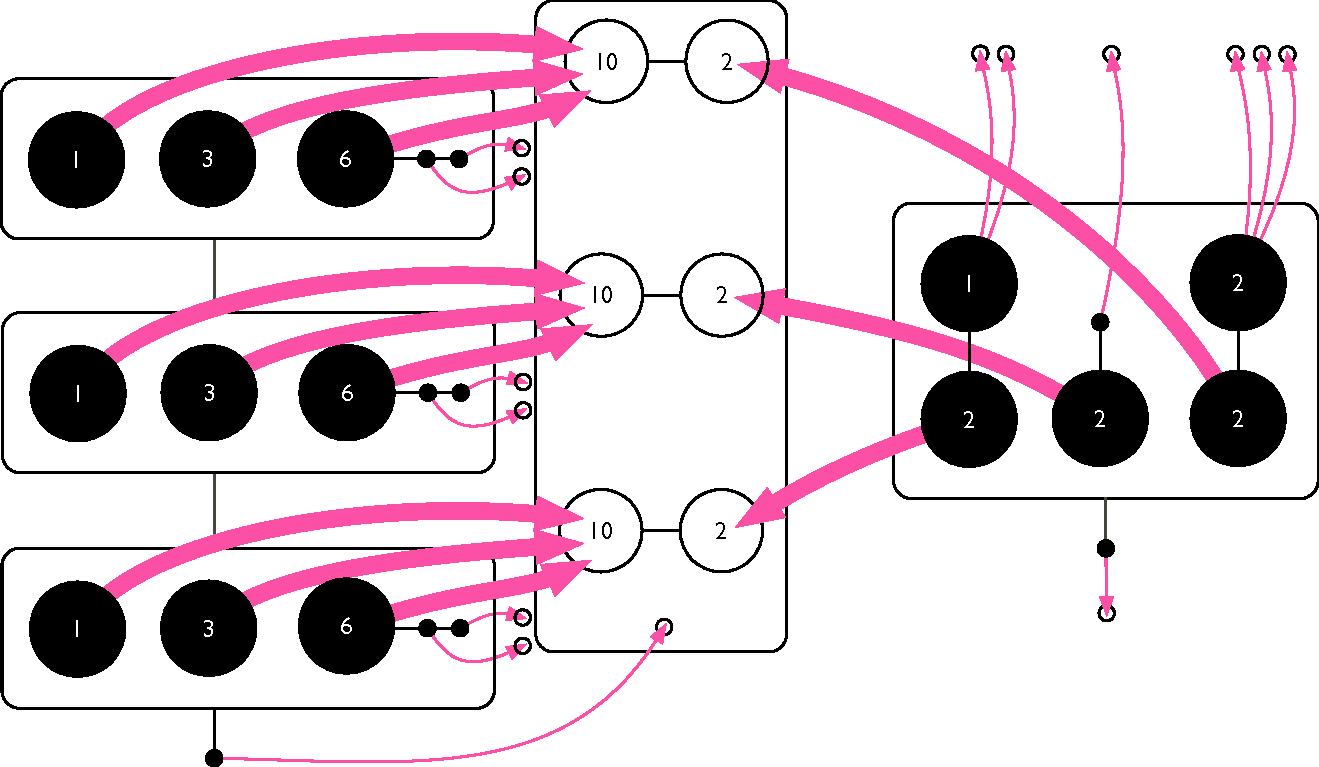
\includegraphics[scale=0.5]{naughty-proofnet.pdf}\end{center}
We have decomposed the edge absorber into 13 individual $\circ$ nodes that are scattered around the diagram, and decomposed some of the other nodes into parts, to make the diagram more legible.

The trick we use to overcome this problem is to multiply all the edge weights and minimum inflow constraints by a constant factor that is large enough to make it impossible for an edge to be freed illegitimately using a naughty wiring. The point here is that as $w$ and $c$ become larger, these naughty wirings use the edges more and more inefficiently. To make this precise, we'll use a little combinatorial lemma:

\begin{lemma}
    A non-empty bipartite forest whose leaves are all in the same part has more vertices in the part that contains the leaves than in the part that doesn't.
\end{lemma}
\begin{proof}
Here a forest is an acyclic graph, a leaf is a vertex that has fewer than two neighbours, and bipartite means the nodes are coloured red and blue in such a way that every arc connects a red and a blue node. Without loss of generality, by symmetry, we assume the leaves are red; we want to show there are more red vertices than blue ones.

It suffices to show this for trees, i.e.\ connected acyclic graphs, since a forest is a union of trees. So take a tree: either all its nodes are red, in which case we are done, or it has some blue non-leaf nodes, in which case pick one to be the root and direct all the edges towards it. Every vertex has a unique successor (or parent) under this orientation, and since the leaves are red and the colours alternate along each path this successor relation determines a surjection from the red nodes onto the blue ones. Since the root has more than one predecessor by hypothesis, this surjection cannot be a bijection, so there must be strictly more red vertices than blue ones.
\end{proof}

Now, a wiring of our gadgets determines a bipartite graph of this sort, in the following way. The blue vertices are going to be the rows of node gadgets, specifically the rows that are linked to more than one edge gadget. (Our aim is to find an upper bound on the number of such rows.) The red vertices are going to be the \emph{columns} of the edge gadgets.

When a row of a node gadget is filled by more than one edge gadget, there must in any case be some pair of edge gadgets that touch opposite sides of the tensor in the node gadget. For each such row, choose some such pair, and add a pair of corresponding arcs to the graph.

This graph must be acyclic by the proof net criterion. So the number of naughtily-filled rows is less than the total number of edge gadget columns, which is three times the number of edges in the constraint graph. It follows that, when constructing a sequent from a constraint graph, we may multiply all our $w$ and $c$ values by a factor $m$ equal to thrice the number of edges. Since we know that fewer than $m$ rows of any node gadget may be filled in a naughty way, and since each edge gadget has a number of rows that is a multiple of $m$, it can never now happen that an edge is released from a node when it ought not to have been.

[TODO: Explain how edge absorbers can be moved about when an edge gadget moves to a different node, so that it doesn't matter how the edge absorbers are attached to the edges in the two proof nets.]


\section*{Remarks}
It is \textsc{pspace}-complete to decide, for a proof net, whether a particular link may be moved. This follows from the \textsc{pspace}-completeness of the configuration-to-edge problem for \textsc{ncl}.

I believe proof equivalence is decidable in linear time for the intuitionistic fragment of \textsc{mll}, which is an interesting (and surprising?) contrast to the classical case. Dominic Hughes and I have an old unfinished draft showing this -- it is basically all Dominic's work, to be honest -- and I think the argument there is sound. There's an attempt at it in Audrey Tan's thesis, which unfortunately contains serious errors. Our draft is an attempt at a correct proof based on Tan's ideas. Does it follow from any correct existing work?

There is an unresolved question about depth-limited formulas, where by depth I mean how deeply nested the boxes are in the diagram. At depth zero -- where no boxes are used, and so every entry in the sequent is a tensor of atoms -- there is a straightforward (but not entirely trivial) linear-time algorithm. The reduction above shows that depth two is \textsc{pspace}-complete. So what happens at depth one? This is an open question.

\bibliography{refs}
\end{document}
